\chapter{Training Strategies}\label{s:train}

This chapter is about all the things I used and did to improve/allow the training of the algorithm, using the datasets described and implemented in the previous chapter, \emph{Datasets}.

\section{Training program used}\label{s:fizyr}

The training program used is a less popular implementation of \maskrcnn. The most popular one, and the one you easily find on Google, is MatterPort.

This one is called keras-maskrcnn and lives on GitHub at the url \emph{https://github.com/fizyr/keras-maskrcnn}.

This below is the brief disclaimer taken directly from his repo:

\begin{quote}[github.com/fizyr/keras-maskrcnn]{hgaiser}
	This repository doesn't strictly implement MaskRCNN as described in their paper. The difference is that their paper describes using a RPN to propose ROIs and to use those ROIs to perform bounding box regression, classification and mask estimation simultaneously. Instead, this repository uses RetinaNet to do the bounding box regression and classification and builds a mask estimation head on top of those predictions.
	
	In theory RetinaNet can be configured to act as a RPN network, which would then be identical to MaskRCNN, but doing so would require more layers and complexity than is actually necessary. Less is more :)
\end{quote}

Keeping this in mind, it actually works quite well and can generalize even with broken datasets, as explained in the previous chapter.

It can be installed quite easily (just follow the guide on the repository).

Some images of the program trained on the COCO dataset [\sref{s:coco}] can be found below.


% --- figure begins ---%
\begin{figure}[H]
	\centering
	\setlength{\tabcolsep}{0.5pt}
	\setlength{\fboxsep}{0pt}%
	\setlength{\fboxrule}{0.1pt}%
	\renewcommand{\arraystretch}{0.6}
	\begin{tabular}{ccc}
		%\multicolumn{1}{c}{Query} & &\multicolumn{5}{c}{Retrieved Images} & &\multicolumn{1}{c}{Query}  & &\multicolumn{5}{c}{Retrieved Images} & &\multicolumn{1}{c}{Query}  & &\multicolumn{5}{c}{Retrieved Images}\\ 
		%1st row----------------------------
		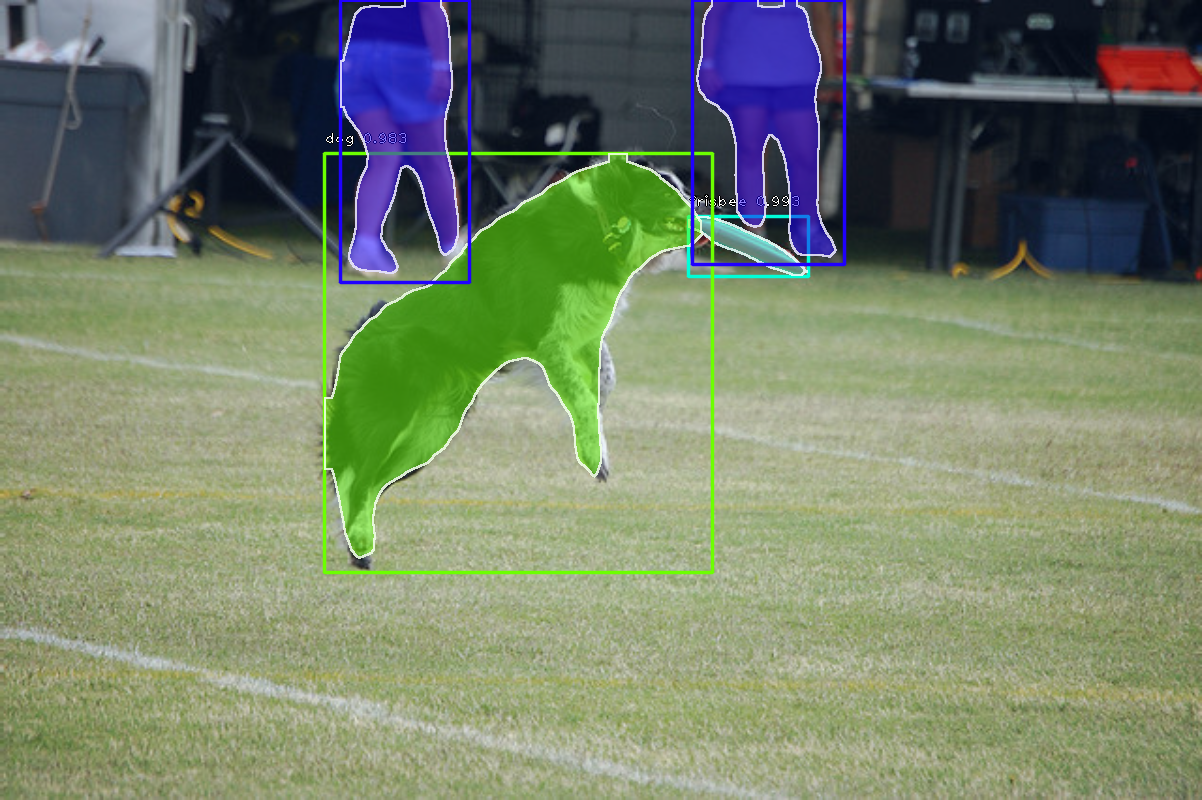
\includegraphics[width=.35\textwidth]{./figures/fizyr/01} & 
		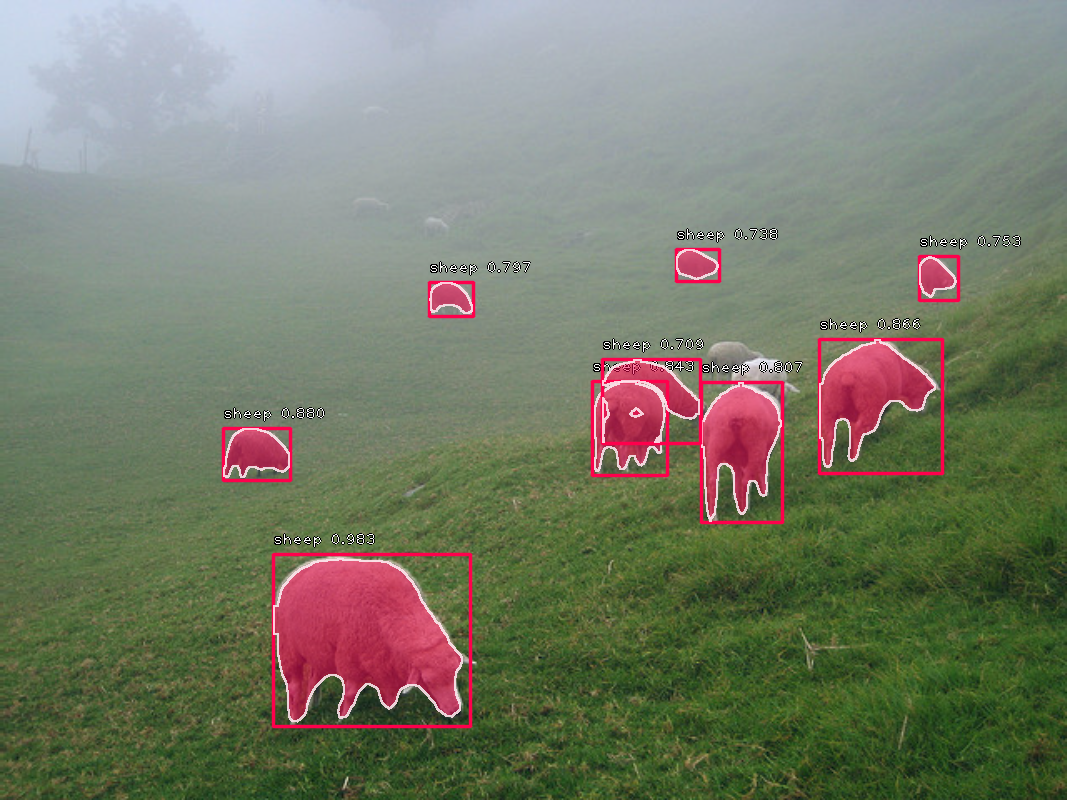
\includegraphics[width=.31\textwidth]{./figures/fizyr/02} &
		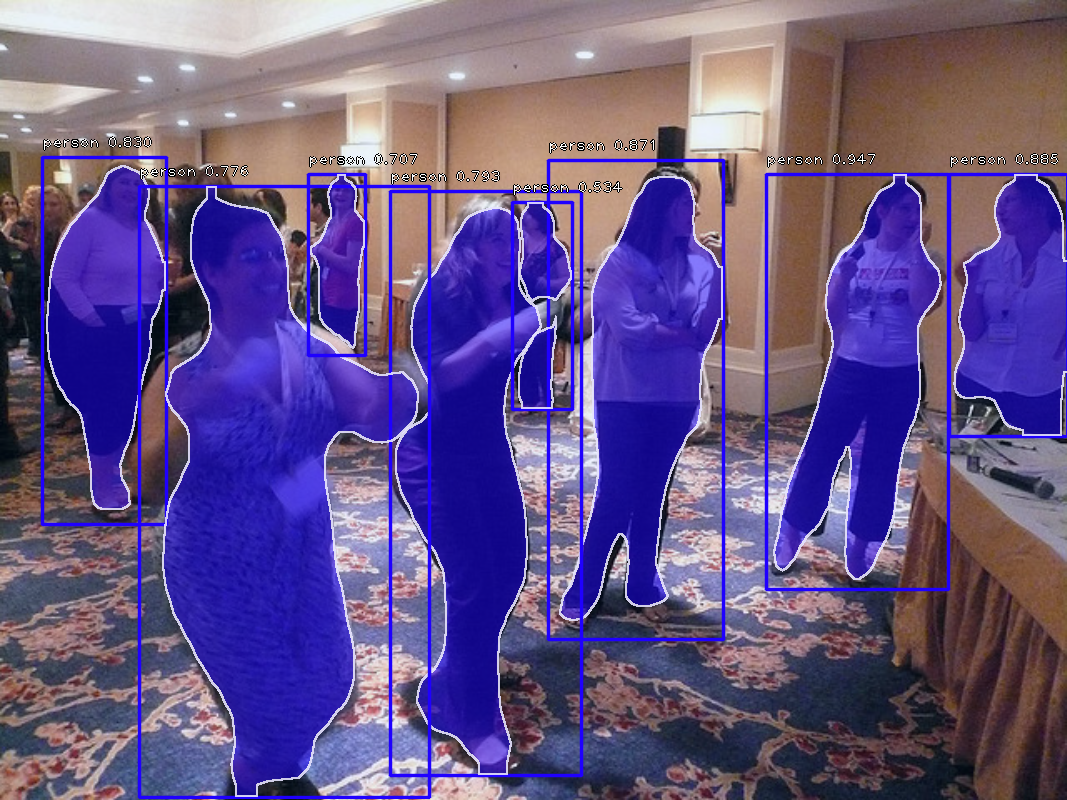
\includegraphics[width=.31\textwidth]{./figures/fizyr/03}\\
	\end{tabular}
	\caption{Results of fizyr's Mask R-CNN based on RetinaNet backbone, trained on COCO.}
	\label{f:fizyr} %% label for entire figure
\end{figure}
% --- figure ends --- % 

The performance results can be found below (note: the closest resembling architecture in the MaskRCNN paper achieves an mAP of 0.336).

\begin{lstlisting}[language=bash]
Average Precision  (AP) @[ IoU=0.50:0.95 | area=   all | maxDets=100 ] = 0.278
Average Precision  (AP) @[ IoU=0.50      | area=   all | maxDets=100 ] = 0.488
Average Precision  (AP) @[ IoU=0.75      | area=   all | maxDets=100 ] = 0.286
Average Precision  (AP) @[ IoU=0.50:0.95 | area= small | maxDets=100 ] = 0.127
Average Precision  (AP) @[ IoU=0.50:0.95 | area=medium | maxDets=100 ] = 0.312
Average Precision  (AP) @[ IoU=0.50:0.95 | area= large | maxDets=100 ] = 0.392
Average Recall     (AR) @[ IoU=0.50:0.95 | area=   all | maxDets=  1 ] = 0.251
Average Recall     (AR) @[ IoU=0.50:0.95 | area=   all | maxDets= 10 ] = 0.386
Average Recall     (AR) @[ IoU=0.50:0.95 | area=   all | maxDets=100 ] = 0.405
Average Recall     (AR) @[ IoU=0.50:0.95 | area= small | maxDets=100 ] = 0.219
Average Recall     (AR) @[ IoU=0.50:0.95 | area=medium | maxDets=100 ] = 0.452
Average Recall     (AR) @[ IoU=0.50:0.95 | area= large | maxDets=100 ] = 0.565
\end{lstlisting}


\section{Splitting the annotations}\label{s:splitting}

Splitting the annotations has been a fun project for me and the script has a really nicely formatted output. The problem has been introduced in \sref{s:ds-org-mn}

The best version was put into the CLI [introduced in the \emph{Datasets} chapter, \sref{s:ds-package}].

So I first thought: I need to preserve the balance of how many annotations in percentace for each type go into each set, and the more images I have in the training dataset, right?

Not right! But before we draw any conclusions, let me explain why.

The initial solution I had thought about was dividing the dataset not by image, but by annotation. That meant that an image could appear both in the training set and the validation set, but on the training set it had \emph{some} annotations, and in the validation set it had \emph{some other} annotations.

That made it easy to check how balanced the training set splitting was, since you could just tell the script to split with a certain probability for each category.

The problem was really clear just as I started training on it: the algorithm would think that the sometimes a bag \emph{is} a bag, and sometimes \emph{it isn't}. So it would naturally be confused and give poor results.

Abandoning this initial thought, I proceeded splitting the annotations the “right way", and I immediately got much better results. The “V1s" were so bad, I didn't even keep them. Also, one thing to note, the performance results depend also on how good quality the validation annotations are. So even though the performance was actually better that what it was written in the AR and AP [explained in \sref{s:trainalg-evalmetrics}], the results were not put into the perspective that the validation file contained only \emph{some} results that were right, so it could not compute the validation evaluation correctly.

\subsection{V1: by annotation}\label{s:splitting-1}

\lstinputlisting[language=Python, firstline=1, lastline=37]{"/Volumes/My Book Cadoppi/DriveUni/3/Thesis cad0p/saveannotationsV1.py"}

In these first lines, I set the percentages, and you can see I correct them if the input is wrong.
I create the training, validation, and test set by copying the common features they have.

\lstinputlisting[language=Python, firstline=39, lastline=48]{"/Volumes/My Book Cadoppi/DriveUni/3/Thesis cad0p/saveannotationsV1.py"}

Here I create the arrays I need to make this program fly through the annotations.

\lstinputlisting[language=Python, firstline=50, lastline=73, breaklines=true]{"/Volumes/My Book Cadoppi/DriveUni/3/Thesis cad0p/saveannotationsV1.py"}

This is the juicy part: for every annotation, it selects randomly (based also on the seed) to which set to append the corresponding annotation, and tells the program to later add the corresponding images to their set (which could be more than one, as explained earlier)

I'll leave out the last part, since it only replaces the img\_ids with their corresponding array and saves the 3 files.

\subsection{V2: by image}\label{s:splitting-2}

I'll start by saying this is the final script, accessible through \lstinline[language=bash]|maskrcnn-modanet datasets arrange| [\fref{f:cli-datasets}]

The first differences easy to notice are that now the program asks for the percentages if they aren't present in the savedvars [\fref{f:cli-savedvars}]. It also copies the original annotations into the ./datasets/coco/annotations/ folder, which is used by the algorithm as a path to get the images and the annotations for training.

I won't put all the code here since the V2 is on GitHub, contrary to V1, but I'll try to explain the best I can and put some necessary snippets here.

I'll put the output of the program, though, as it is similar in form to V1, but of course not on GitHub (I'm not using interactive notebooks).

\begin{figure}[H]
	\centering
	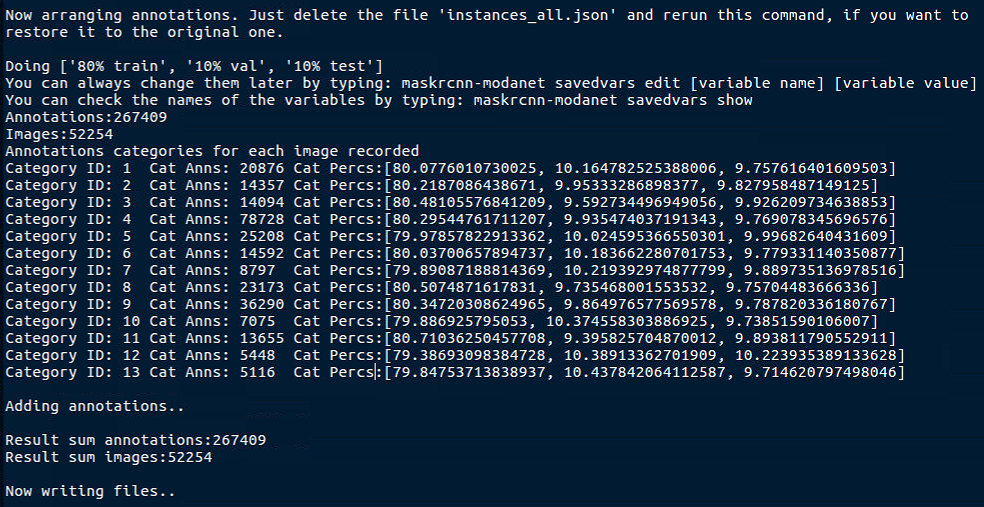
\includegraphics[width=\linewidth]{figures/anns/bestfixed}
	\caption{The datasets arrange function output for the package maskrcnn-modanet}
	\label{f:anns-bestfixed}
\end{figure}

We can see the difficulty of creating the program is proportional to the spanning arrays that we need to make the program fly (initially it would take literally hours, before I optimized it and now it runs in a few seconds!)

Here are some used in V2:

\lstinputlisting[language=Python, breaklines=true, firstline=84, lastline=98]{/Users/piercarlocadoppi/Documents/GitHub/maskrcnn-modanet/maskrcnn_modanet/arrange_annotations.py}


\section{Fixing the annotations!}\label{s:fixing}

Fixing the annotations required a lot of patience and perseverance.

It's a bit of a guessing game since, as described in \sref{s:ds-mn-fix}, unfortunately \modanet is flawed by a serious bug on footwear and boots, that strongly limits the performance of retrieval of results.

The way I set out to solve it, I tried to find the bouding boxes that were overlapped and had the same label, then I looked into the shapes, to see if they had shapes present in both annotations (I went through a double loop for looking through all the annotations one vs. one).

18 thousand boxes fixed, 35 thousand not totally, the rest I was not able to fix. But this was good enough for the training algorithm to learn the concept and texture of footwear and shoes, so it all went well.

I did of course many revisions, trying to learn what the annotations had wrong and how to fix it.

Back to the code, I deleted the double shapes from one of the annotations, with criteria such as how much that shape is fit to that box, or if it is even contained (meny weren't).

Here's a snippet:

\lstinputlisting[language=Python, breaklines=true, firstline=314, lastline=330]{/Users/piercarlocadoppi/Documents/GitHub/maskrcnn-modanet/maskrcnn_modanet/fix_annotations.py}

There was usually a wrong box and a correct one, so I tried to find: which one is the correct one?

If a shape in annotation 1 is not contained in annotation 1 and a shape in annotation 2 is instead contained (in annotation 2), that means the bbox for the annotation 1 is probably wrong!

Then I moved the boxes trying to keep the proportions (so I only translated the bbox).

Finally, I moved the lonely annotations (annotations that do not fit anywhere) to a newly made mask, and moved around shapes that were fit for another box.

\subsection{Fixing Results}\label{s:fixing-r}

Apart from \fref{f:modanet-fix}, there are many other cases in which annotations are now better segmented and bboxes moved around better.

% --- figure begins ---%
\begin{figure}[H]
	\centering
	\setlength{\tabcolsep}{0.5pt}
	\setlength{\fboxsep}{0pt}%
	\setlength{\fboxrule}{0.1pt}%
	\renewcommand{\arraystretch}{0.6}
	\begin{tabular}{ccc}
		%\multicolumn{1}{c}{Query} & &\multicolumn{5}{c}{Retrieved Images} & &\multicolumn{1}{c}{Query}  & &\multicolumn{5}{c}{Retrieved Images} & &\multicolumn{1}{c}{Query}  & &\multicolumn{5}{c}{Retrieved Images}\\ 
		%1st row----------------------------
		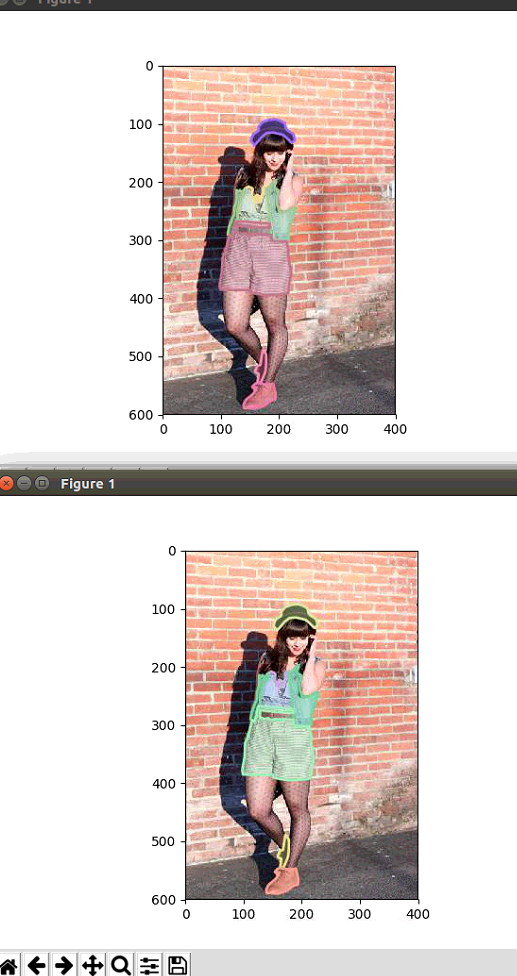
\includegraphics[width=.31\textwidth]{./figures/modanetfix/segm1} & 
		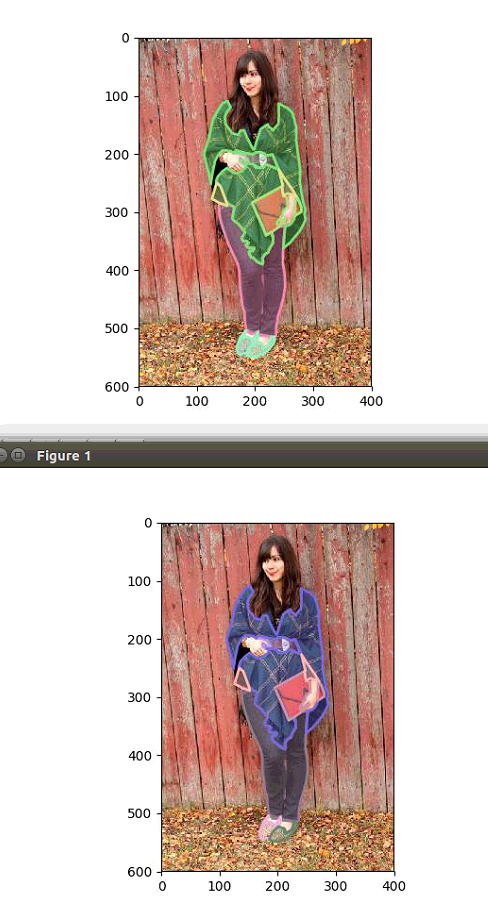
\includegraphics[width=.31\textwidth]{./figures/modanetfix/segm2} &
		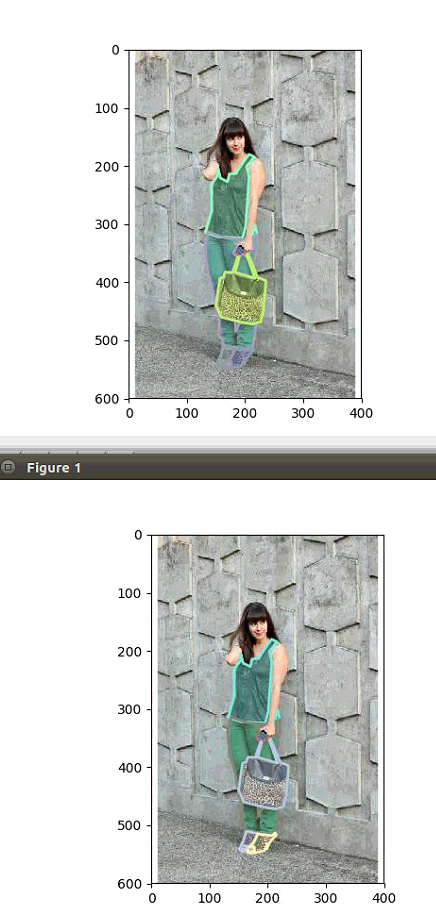
\includegraphics[width=.31\textwidth]{./figures/modanetfix/segm3}\\
	\end{tabular}
	\caption{Qualitative results of new annotations' fix for ModaNet. The images above are the original, below the fixed ones.}
	\label{f:modanet-fix2} %% label for entire figure
\end{figure}
% --- figure ends --- % 

\section{Parameters and Tests}\label{s:parameters-and-tests}

\subsection{Invalid Indexes}\label{s:indexes-invalid}

Just as I started, and for a while, I had this problem: for the first 5 epochs of training, the program would tell me that there were invalid indexes. I hadn't yet built the very useful tool for analyzing the annotations, so with Leonardo we looked with the debugger to try and find what caused the bug. We had just discovered a piece of the “fixing the annotations" puzzle.

Some bboxes (bounding boxes) were going off the charts, which means they were going out of the bounds of the image.

So I “fixed" it by resizing the boxes during training to make them fit. I have to acknowledge than, even with the annotations now fixed (not only the indexes thing), some of them are still not fixed so I have left the “fix" active. While previously it was more of 1 in 5 images, now it is about 1 in 20, I have to say in my favour!

It's clear why they only happened up until epoch 5: the images are about 50k, the steps per epoch are 10k, and the \emph{batch size} -- that is, how many images are processed per step -- is 1. And the generator deleted the invalid annotations when it saw them, so after it goes through all the images of course it does't throw any errors anymore.

\subsubsection{Initial Working Test}

This was done when I had just developed the new annotations splitting algorithm, V2. 

Keep in mind the results below are not in relation to the fixed annotations, so they are not very important by themselves now. Keep in mind also that the new fixed annotations tend to improve the evaluation metrics of previous models.

I'll just post the photo of the last epoch.

\begin{figure}[H]
	\centering
	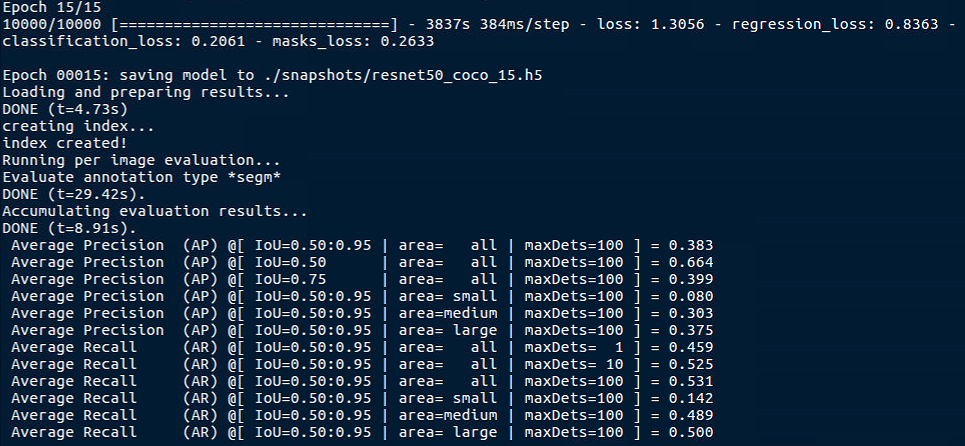
\includegraphics[width=\linewidth]{figures/train/initial}
	\caption{Initial training with Mask R-CNN (fizyr implementation) and ModaNet annotations}
	\label{f:train-initial}
\end{figure}


\subsubsection{28/50 Epochs test}

This test was the one while I was trying to solve how to make the package and fix the annotations.
It was stopped because I was hogging the shared computer too much :)

I got the best results from this one (apart from footwear) because it had a greater LR (learning rate) than the fixed indices 28 (because it was not supposed to stop at 28).

The segmentation was almost perfect and very precise. In fact, the image on the introduction is from this model!

\begin{figure}[H]
	\centering
	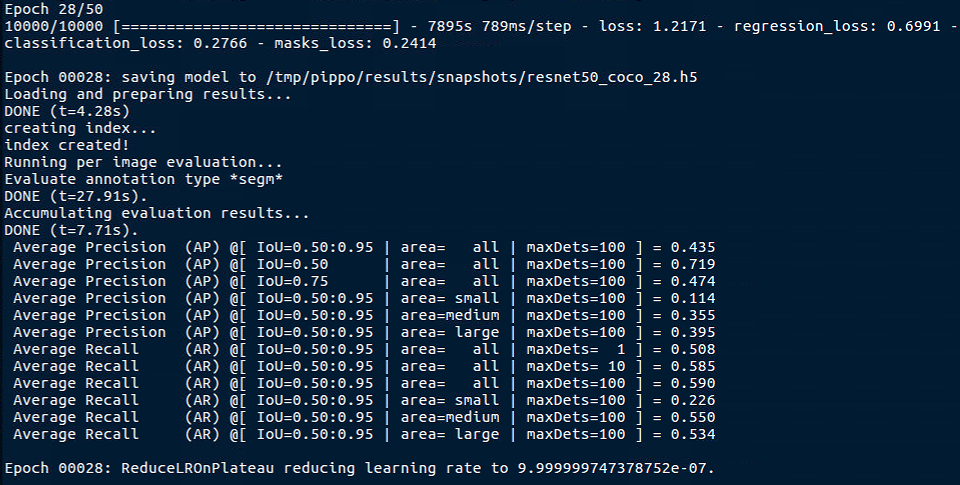
\includegraphics[width=\linewidth]{figures/train/28-50}
	\caption{28 epochs out of 50 with the indices fixed (bounding boxes resized) and ModaNet annotations}
	\label{f:train-28-50}
\end{figure}

\subsubsection{Resuming from 28 Short Test}

I discovered here that resuming from a snapshot keeps the loss function artificially low. I can't explain this since I never understood it really well, but it seems like loading from a snapshot isn't the same thing as just letting the training go without stopping. Qualitative results were especially affected, the segmentation was very bad, just like when a new training starts and the algorithm has to adjust the weights all-over again.

\begin{figure}[H]
	\centering
	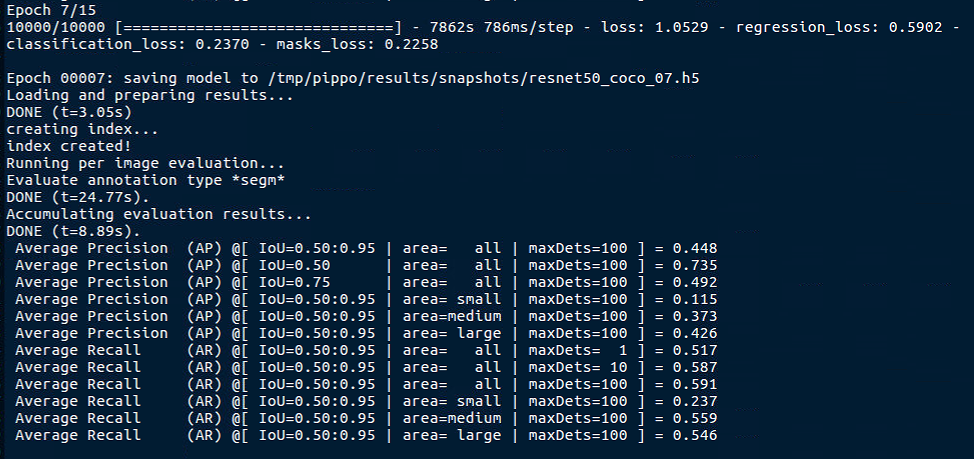
\includegraphics[width=\linewidth]{figures/train/28-50resuming7}
	\caption{7 epochs with the indices fixed (bounding boxes resized) and ModaNet annotations}
	\label{f:train-28-50resuming7}
\end{figure}

\subsection{Fixed Indexes}

As explained in \sref{s:indexes-invalid}, we allowed the invalid annotations by simply resizing the bounding boxes to the max height/width of the image.

\subsubsection{28 Epochs Full Test}\label{s:train-28fixedindices}

\begin{figure}[H]
	\centering
	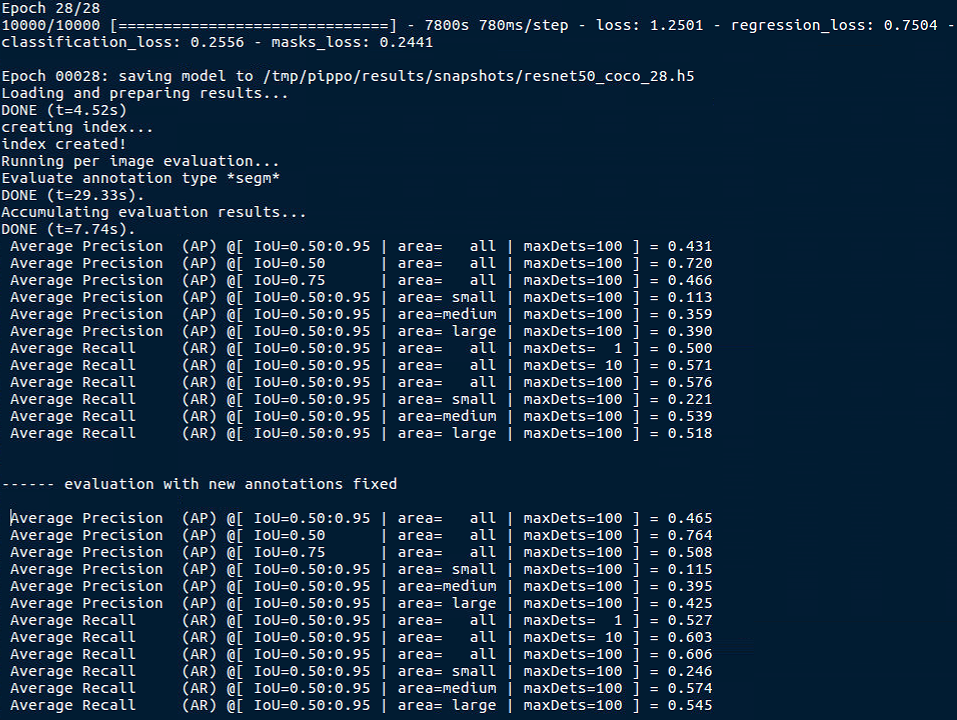
\includegraphics[width=\linewidth]{figures/train/28fixedindices}
	\caption{28 epochs with the indices fixed (bounding boxes resized) and ModaNet annotations}
	\label{f:train-28fixedindices}
\end{figure}



\subsubsection{15 Epochs No Weights Test}

This was an hopeless test: of course it would perform worse than the one pretrained on ImageNet, \sref{s:imagenet}, weights.

But it was interesting since it put into perspective just how helpful is to start from pretrained weights, even though what we were trying to solve here is very different from the ImageNet dataset. This shows us that the algorithm learns more easily to understand high level concepts if it already knows how to distinguish (in general) one object from another.

\begin{figure}[H]
	\centering
	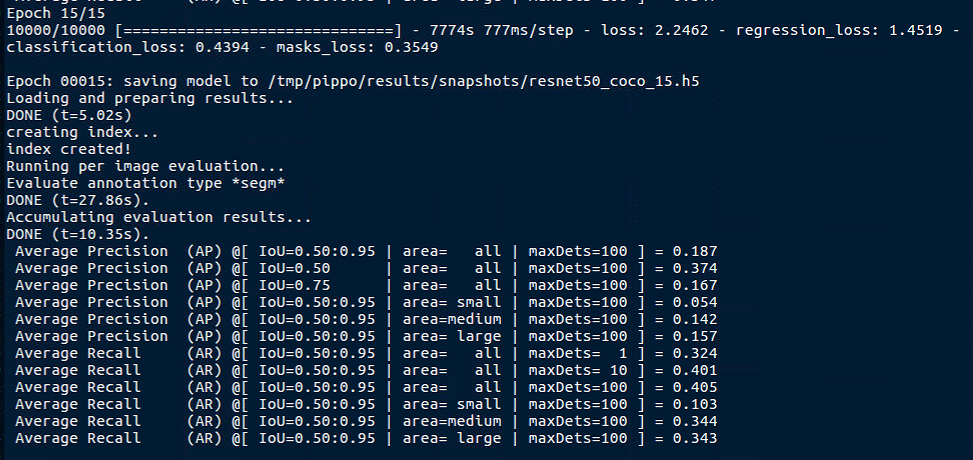
\includegraphics[width=\linewidth]{figures/train/15noweights}
	\caption{15 epochs initialized with no weights with the indices fixed (bounding boxes resized) and ModaNet annotations}
	\label{f:train-15noweights}
\end{figure}

\subsubsection{15 Epochs Default Settings Test}

Just for the sake of comparison, let's compare the 15 epoch no weights with the 15/28 epoch of \sref{s:train-28fixedindices}.

\begin{figure}[H]
	\centering
	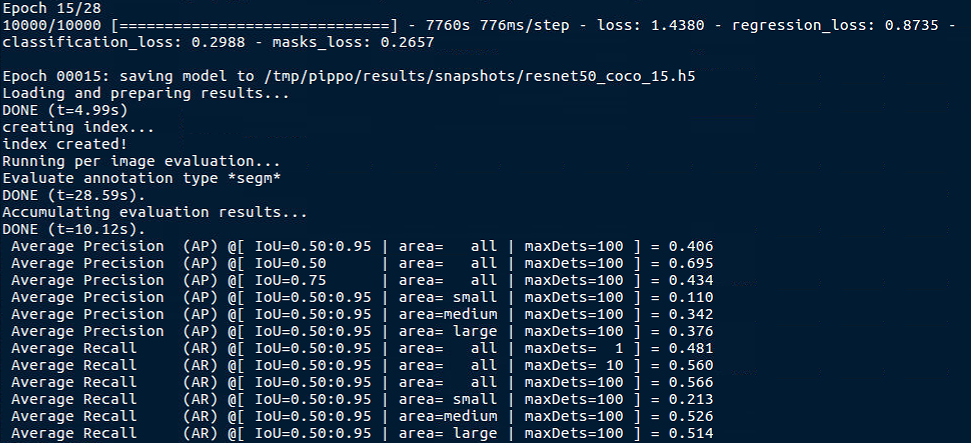
\includegraphics[width=\linewidth]{figures/train/15-28fixedindices}
	\caption{15 epochs out of 28 with the indices fixed (bounding boxes resized) and ModaNet annotations}
	\label{f:train-15-28fixedindices}
\end{figure}

You can see just how much better it is in every direction you look at it. Every metric is better. I would have shown you some qualitative results (e.g. examples of images), but unfortunately some data was lost as a consequence of a computer crash caused by lack of free RAM available.

\subsubsection{10 Epochs Default Settings Test}

Another similar test, but after the restart of the computer, so I can show you some images!

But first the performance evaluation:

\begin{figure}[H]
	\centering
	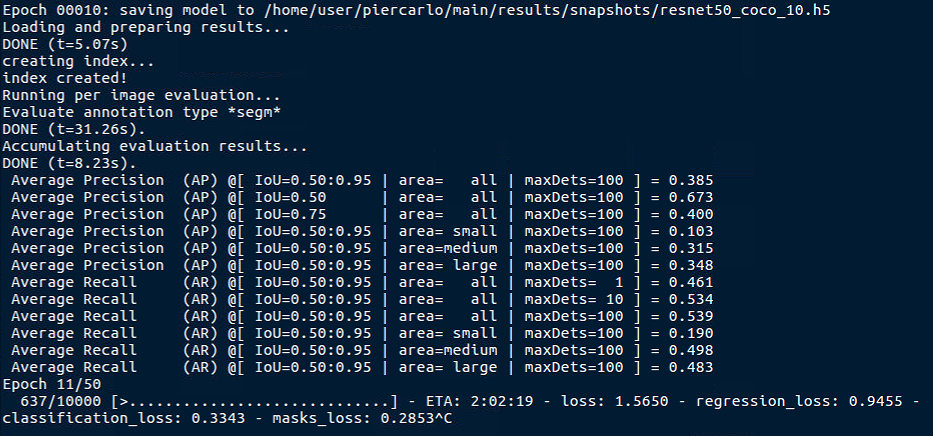
\includegraphics[width=\linewidth]{figures/train/10-50fixedindices}
	\caption{15 epochs out of 50 (stopped before) with the indices fixed (bounding boxes resized) and ModaNet annotations}
	\label{f:train-10-50fixedindices}
\end{figure}

We can see it's reasonably similar to the one in the section above. (it's actually pretty close).



\subsection{Fixed Annotations}

Finally found the cause for the footwear poorly performing, I went on at full speed to see the changes.

\subsubsection{8 Epochs Default Settings}

Epoch 8/15
10000/10000 [==============================] - 8367s 837ms/step - loss: 1.6431 - regression-loss: 1.0738 - classification-loss: 0.2492 - masks-loss: 0.3201

\begin{figure}[H]
	\centering
	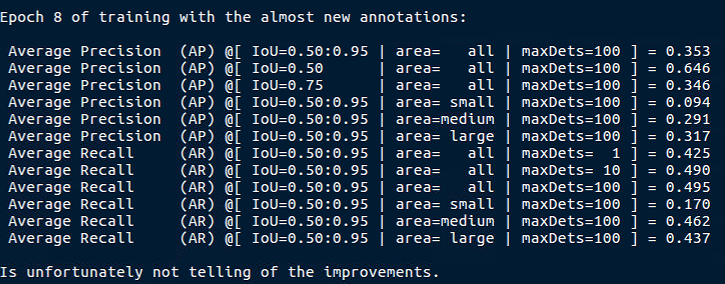
\includegraphics[width=\linewidth]{figures/train/8almostnew}
	\caption{8 epochs out of 50 (stopped before) with the annotations almost fixed (the program was still in developement but I wanted to see preliminary results) and ModaNet annotations}
	\label{f:train-8almostnew}
\end{figure}


\subsubsection{7 Epochs from previous snapshot with improved annotations}

Building up on the previous model certainly helps, even though we have seen that it does not make much of a difference.

\begin{figure}[H]
	\centering
	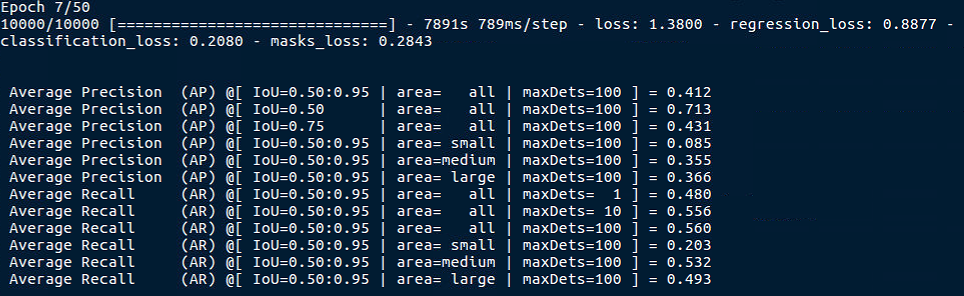
\includegraphics[width=\linewidth]{figures/train/7afteralmostnewwrongdoubleadded}
	\caption{8 epochs out of 50 (stopped before) with the annotations almost fixed (the program was still in developement but I wanted to see preliminary results) and ModaNet annotations}
	\label{f:train-7afteralmostnewwrongdoubleadded}
\end{figure}

The results have mainly improved because of the new improvements in the annotations. Reminder: the evaluation is calculated using the validation dataset, that changed since the annotations changed.

\subsubsection{13 Epochs from previous snapshot with wrongly added double annotations deleted}

\begin{figure}[H]
	\centering
	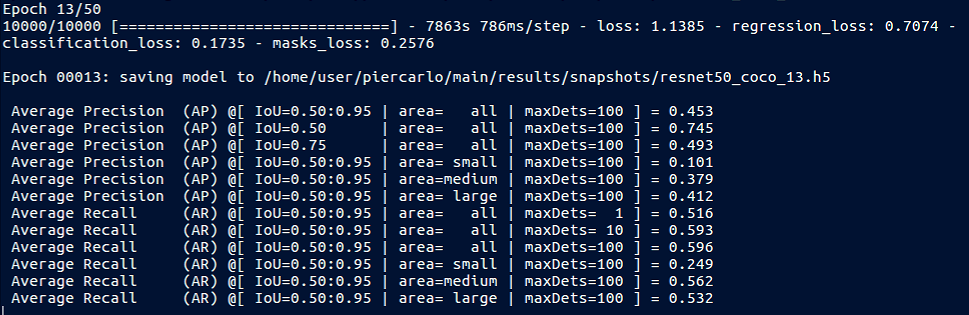
\includegraphics[width=\linewidth]{figures/train/13afterafternewannotations}
	\caption{13 epochs out of 50 (stopped before) with the annotations fixed (deleted mistakenly readded double annotations at the last point in the script) and ModaNet annotations}
	\label{f:train-13afterafternewannotations}
\end{figure}

This result is really pretty good and can be compared to the 28 fixed indices one. (with the same annotations' evaluation). This shows that training from a snapshot gives you some advantages, after all. Image comparisons in the next chapter, \sref{s:r}.

\subsubsection{3 Epochs from COCO weights with same annotations as last one}

the command to train:

\lstinline[language=bash, breaklines=true]|maskrcnn-modanet train --epochs 50 --workers 0 --batch-size 1 --weights /home/user/piercarlo/resnet50_coco_v0.2.0.h5 coco|

The loss starts not too high, just 4.x

\begin{figure}[H]
	\centering
	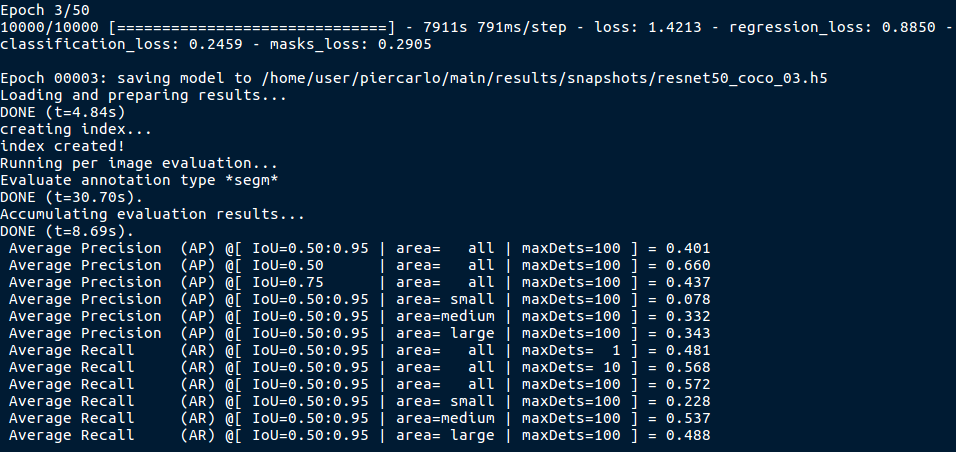
\includegraphics[width=\linewidth]{figures/train/3coconew}
	\caption{3 epochs out of 50 with the annotations fixed (deleted mistakenly readded double annotations at the last point in the script) and the COCO pretrained model. Preliminary results.}
	\label{f:train-3coconew}
\end{figure}

It is looking really good, especially since it is so early in the training.
